This section shows the measurements obtained with the TRITIUM-IFIC 0 prototype during its installation in the Nuclear Radiation Laboratory at IFIC, the design of which was explained in section \ref{subsec:TritiumIFIC0}.

As stated in section \ref{subsec:TritiumIFIC0}, a statistically significant number of events was not obtained when the prototype was read with two PMTs in time coincidence. To overcome this problem, a single PMT measurement was taken using the electronic chain configuration shown in figure \ref{subfig:ElectronicConfiguraiton1PMT}. The energy spectra were measured for both, the signal and background prototypes, which are shown in Figure \ref{subfig:SignalBackgroundEnergySpectraTritiumIFIC0}. As it was mentioned in section \ref{subsection:TritiumIFIC0}, the signal prototype was filled with a tritiated water solution with an activity of $99.696~\kilo\becquerel/\liter$ and the background prototype was filled with ultrapure water.

\begin{figure}[h]
 \centering
  \subfloat[Signal and background energy spectra.]{
   \label{subfig:SignalBackgroundEnergySpectraTritiumIFIC0}
    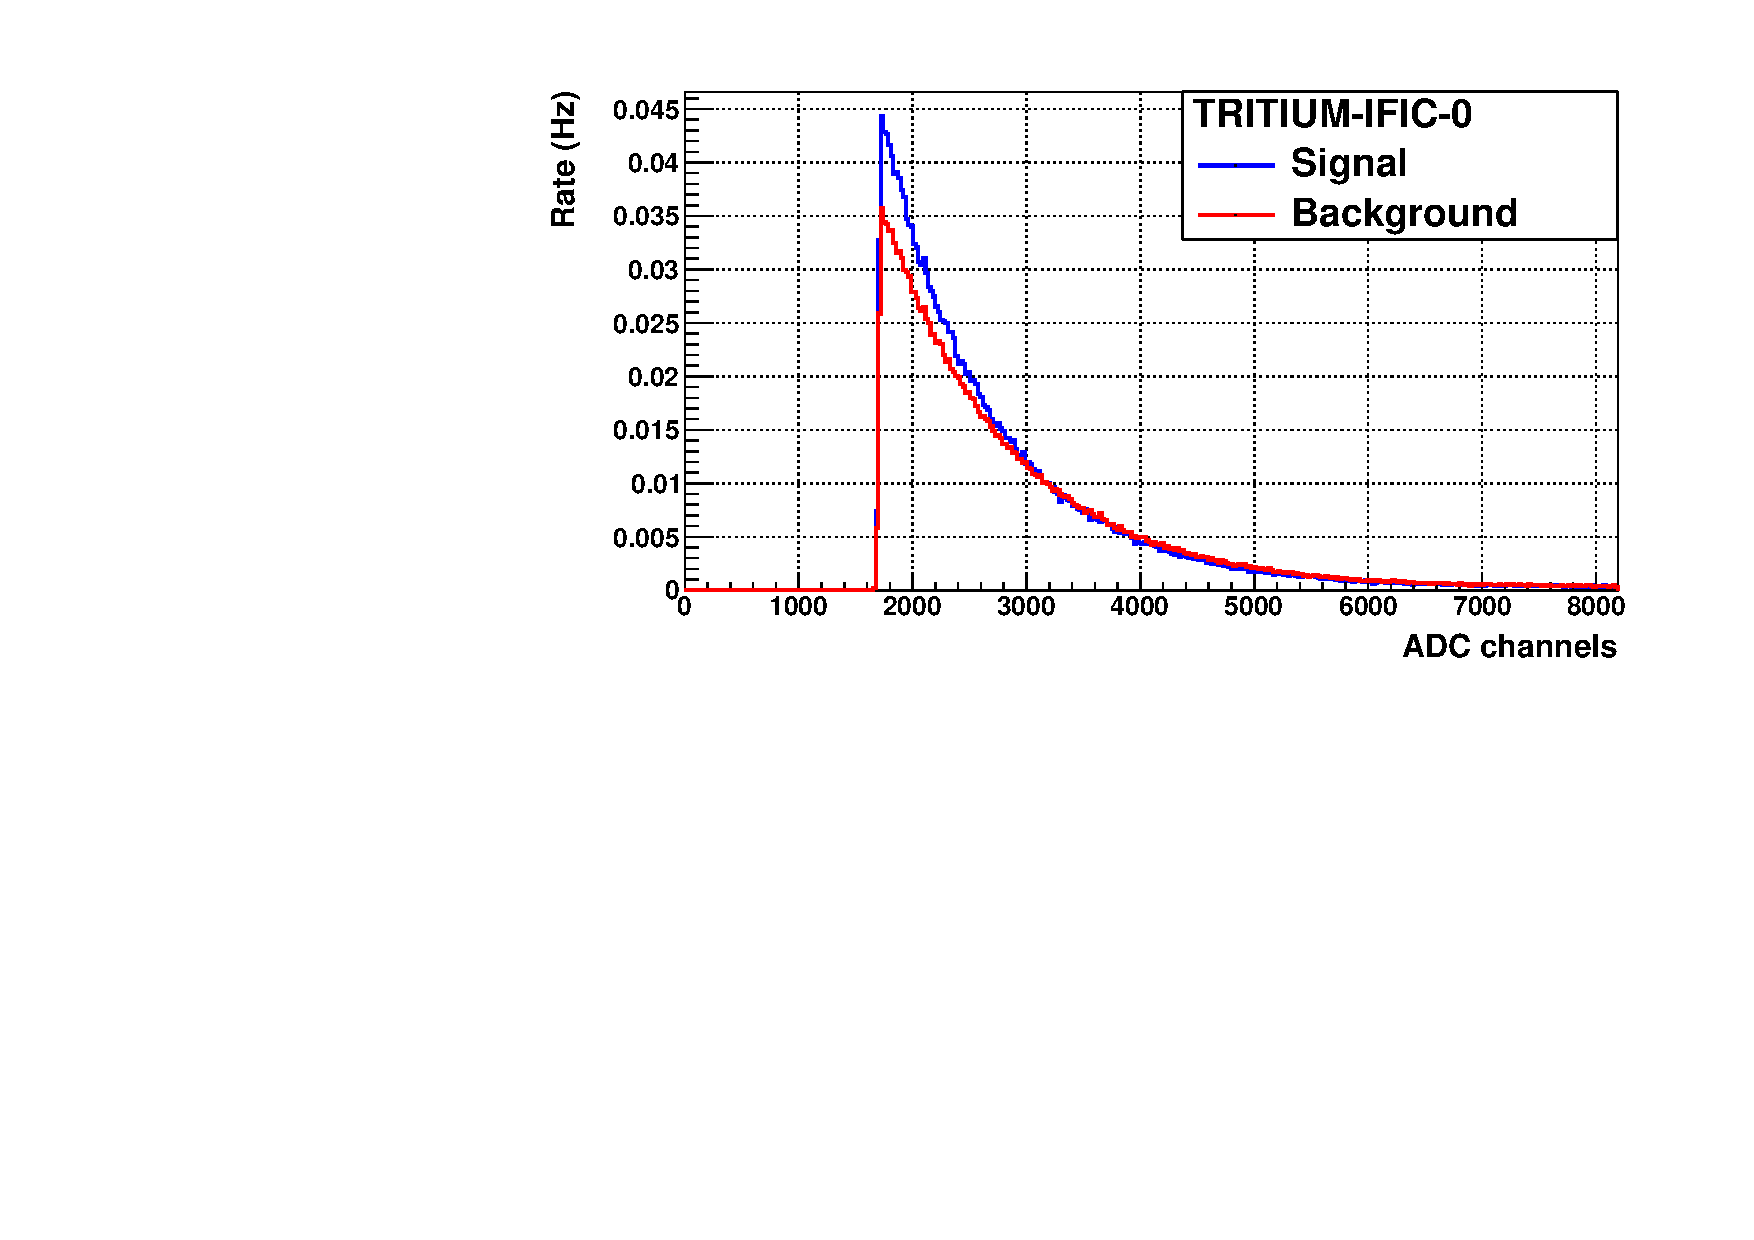
\includegraphics[width=0.73\textwidth]{7ExperimentalResultsDetectors/71ExperimentalResultsLaboratory/711TritiumIFIC0/TritiumIFIC0Signals.pdf}}
   \newline
  \subfloat[Tritium energy spectrum.]{
   \label{subfig:TritiumEnergySpectraTritiumIFIC0}
    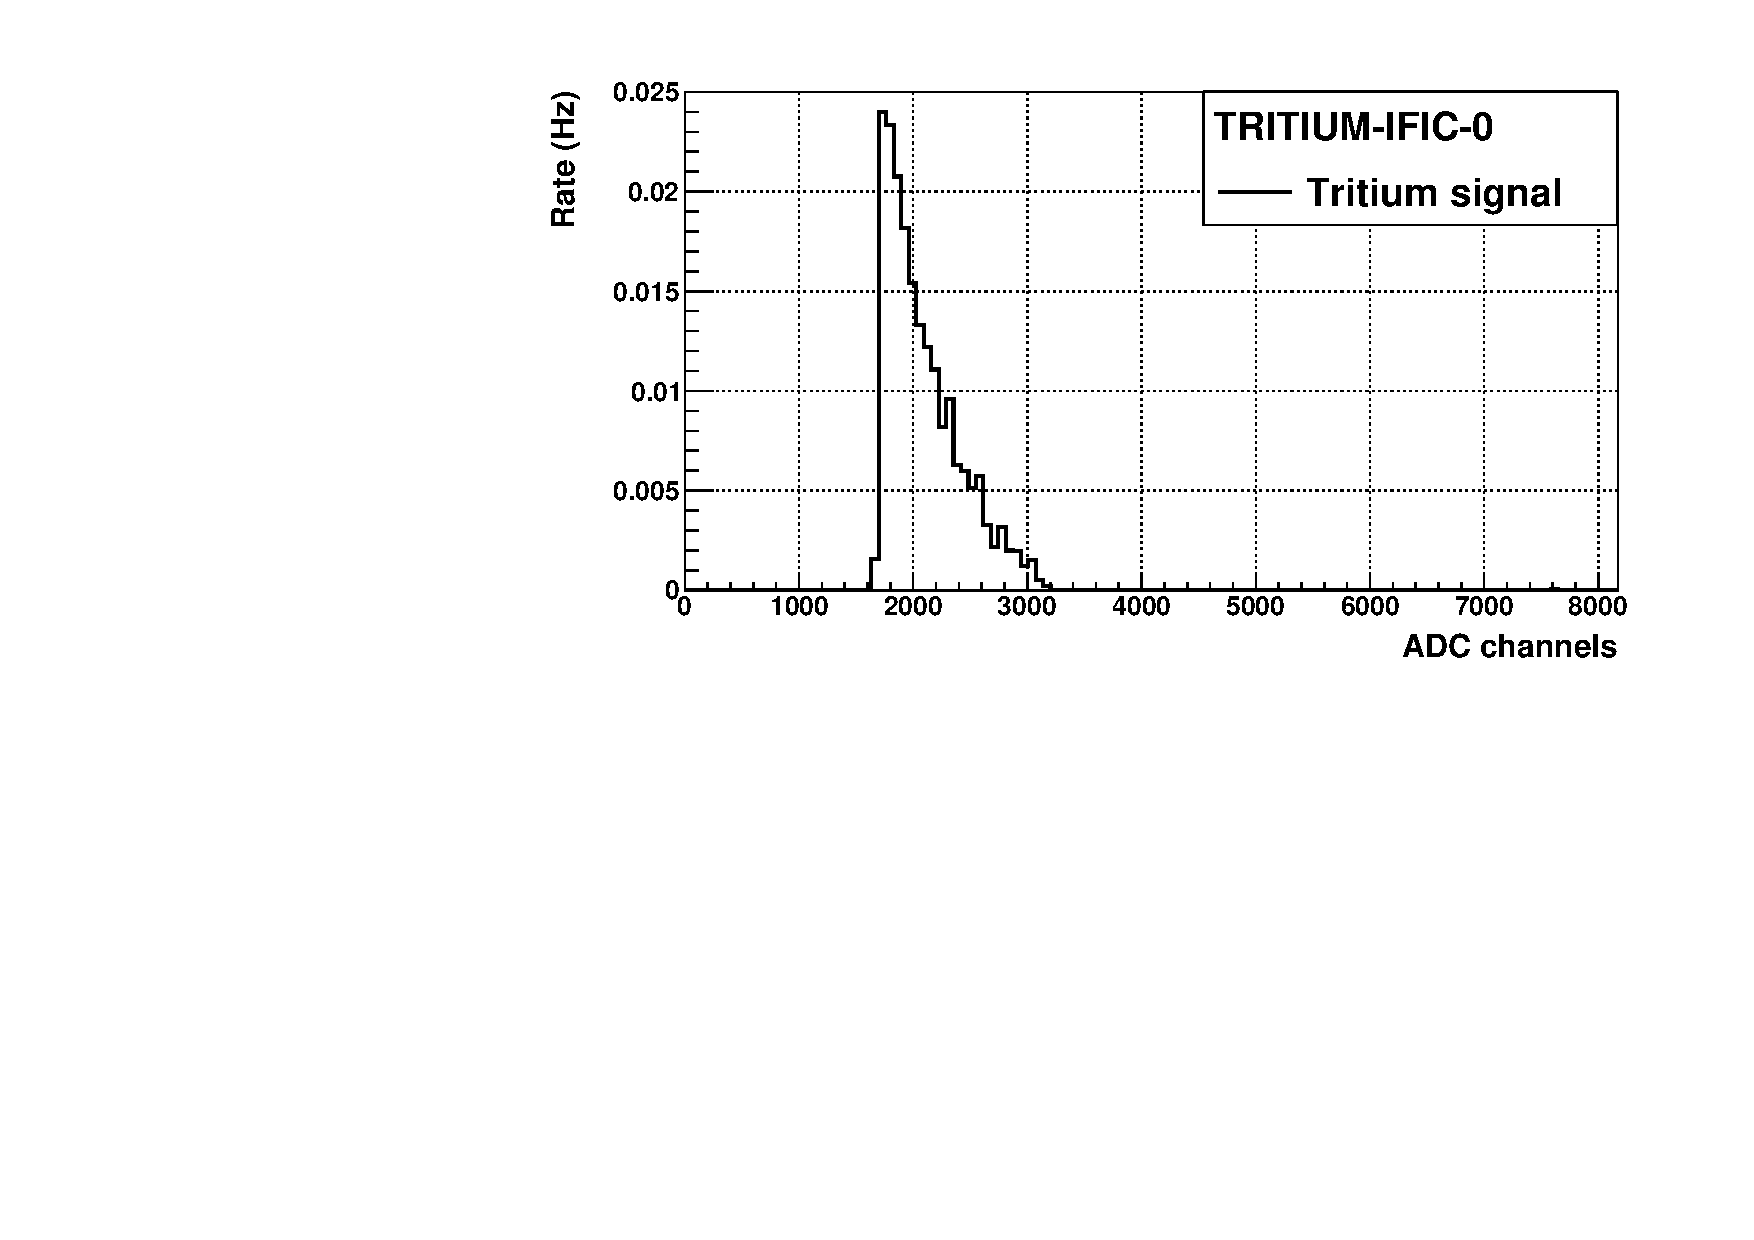
\includegraphics[width=0.73\textwidth]{7ExperimentalResultsDetectors/71ExperimentalResultsLaboratory/711TritiumIFIC0/TritiumIFIC0ClearRebin.pdf}}
 \caption{Energy spectra experimentally measured with TRITIUM-IFIC 0 prototype.}
 \label{fig:EnergySpectraTRITIUMIFIC0}
\end{figure}

%\begin{figure}[htbp]
%\centering
%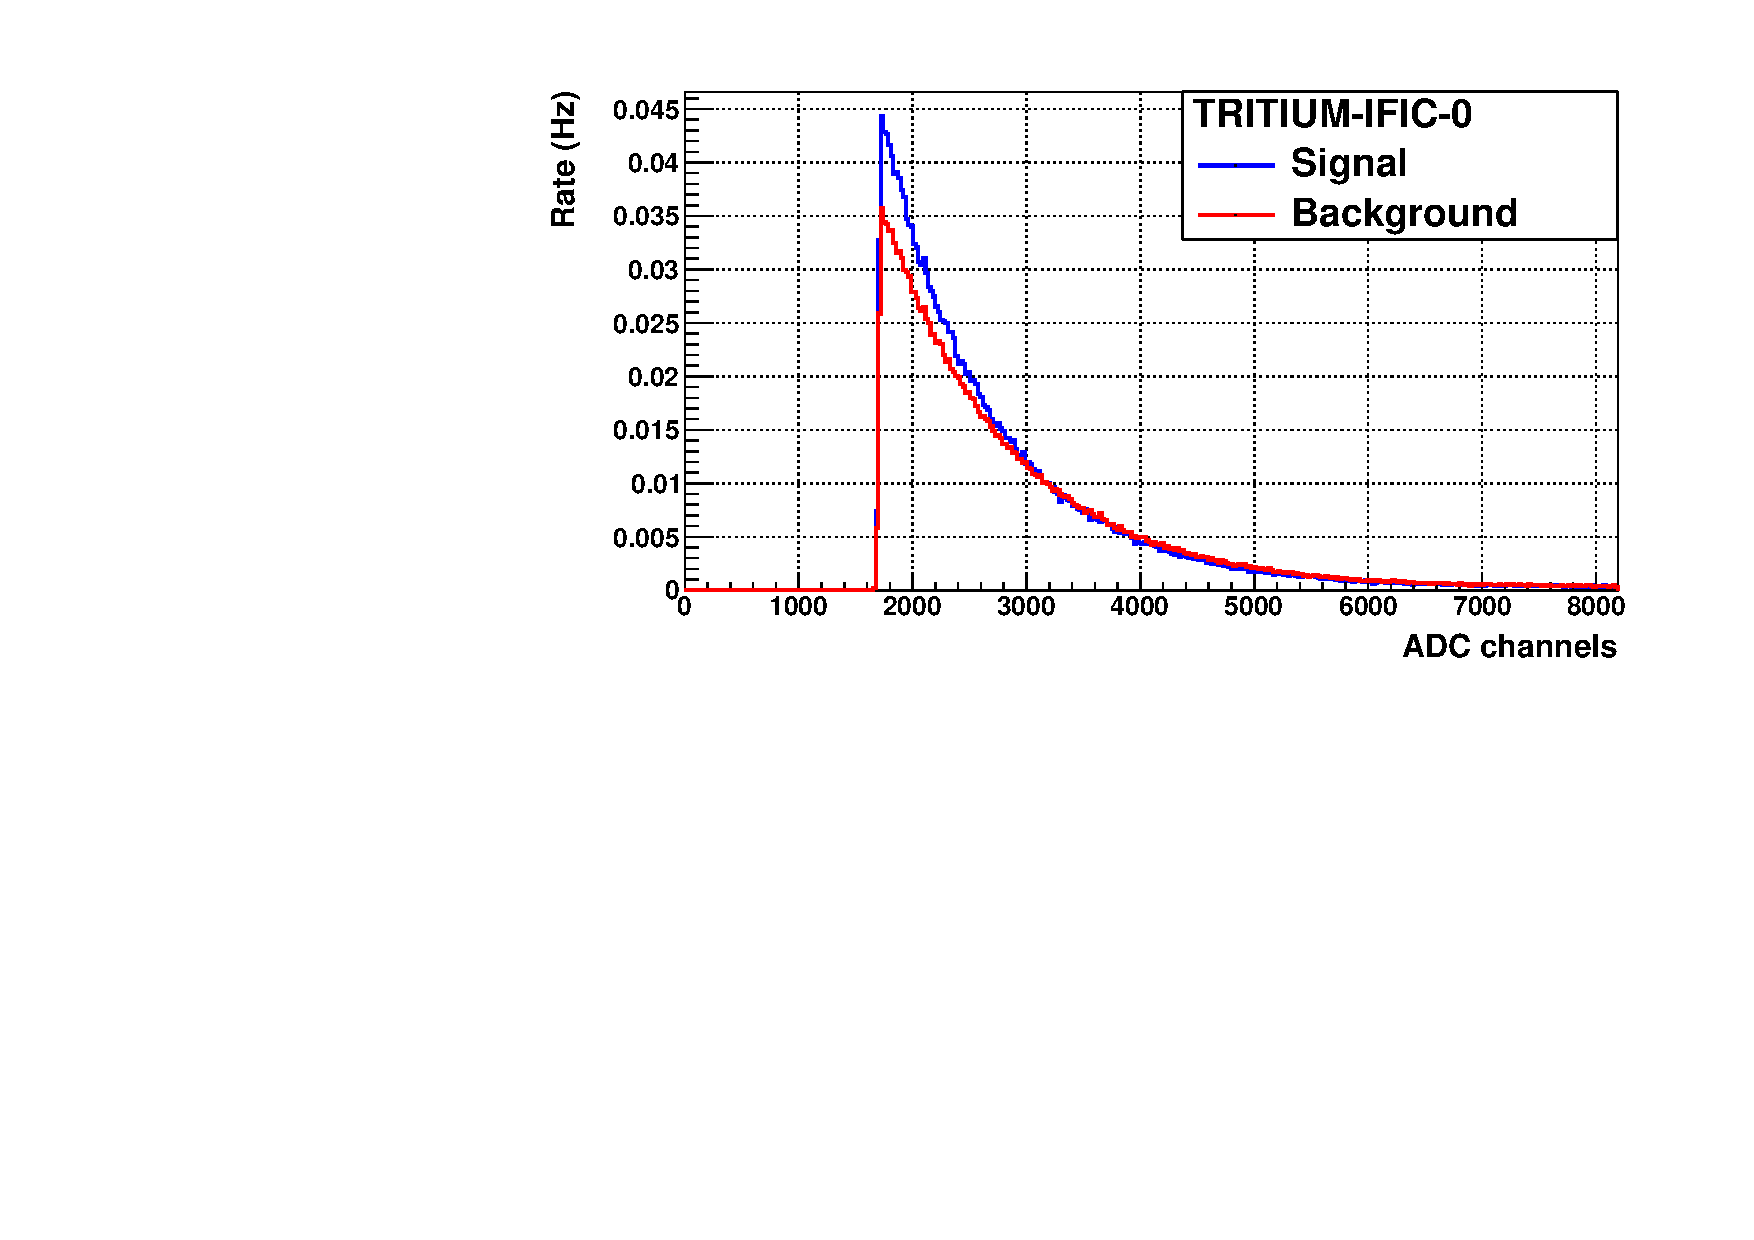
\includegraphics[scale=0.6]{7ExperimentalResultsDetectors/71ExperimentalResultsLaboratory/711TritiumIFIC0/TritiumIFIC0Signals.pdf}
%\caption{Energy spectra experimentally measured with TRITIUM-IFIC 0 prototype.).\label{fig:EnergySpectrumTritiumIFIC0}}
%\end{figure}

In this figure, a difference between both energy spectra is clearly visible, which correspond to the energy spectrum of tritium, Figure \ref{subfig:TritiumEnergySpectraTritiumIFIC0}. A number of counts per second of $2.27 \pm 0.06$ and $2.06 \pm 0.06$ was obtained for the both measurements, signal and background, respectively. Therefore, $0.21$ counts per second was obtained for the tritiated water source used.

The tritium detection efficiency obtained for this prototype is $(2.11 \pm 0.85)\cdot{} 10^{-3}~ \frac{\text{c}/\second}{\kilo\becquerel/\liter}$, which is calculated from the quotient of both, the counts per second measured and the specific activity of the tritium liquid source used.

Comparing with the detectors developed so far by other experiments, Table \ref{tab:PlasticScinTritium} the efficiency obtained is of the order of the detectors the worst results, obtained by Moghissi and Muramatsu. 

As we explained in section \ref{sec:StateOfTheArt}, the efficiency of scintillating detectors scales with the active area of the scintillator used. Therefore, to compare the efficiency with oher detectors and with other prototypes developed in TRITIUM experiment, the specific efficiency of this prototype is calculated, the value of which is $(9.59 \pm 3.88)\cdot{} 10^{-6}~ \frac{\text{c}/\second}{\kilo\becquerel/\liter}\frac{1}{\cm^{2}}$.

As can be seen in the Table \ref{tab:PlasticScinTritium} the specific efficiency is a little bit larger than the detectors with the worsen specific efficiency developed up to now, Muramatsu and Moghissi. This fact can be explained with the loss of photons produced in the curve of the fiber bunch, discussed and experimentally demostrated in section \ref{subsec:TritiumIFIC0}.


%Teniendo en cuenta las efficiencias de los diferentes elementos utilizados (fibras de 20 cm (efficiencia de detección y colleccion), PMTs (efficiencia de photodetección))... las cuentas que deberíamos haber obtenido es de, dando lugar a una efficiencia de XXXX... Se acerca bastante al valor esperado.